\section{Automatización 1: topología de red}

Se realizó la automatización de la topología de red utilizando el protocolo LLDP, el cual permite a los dispositivos de red anunciar su identidad y capacidades a otros dispositivos vecinos. Esto facilita la creación de un mapa de red dinámico y actualizado en tiempo real.

\begin{itemize}
    \item Paso 1: habilitar LLDP
    
\begin{lstlisting}[style=terminal]
system-view
lldp enable
return
save
\end{lstlisting}




\item Paso 2: verificar los vecinos

\begin{lstlisting}[style=terminal]
display lldp neighbor brief
\end{lstlisting}


\begin{figure}[H]
    \centering
    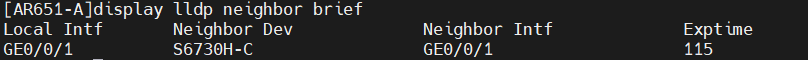
\includegraphics[scale= 0.9]{Pictures/LLD1.png}
    \caption{Confirmación de vecinos de LLDP en el Router A}
    
\end{figure}


\begin{figure}[H]
    \centering
    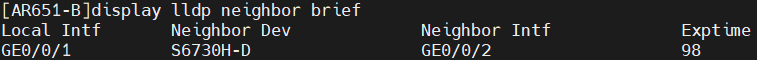
\includegraphics[scale= 0.9]{Pictures/LLD4.png}
    \caption{Confirmación de vecinos de LLDP en el Router B}
    
\end{figure}

\begin{figure}[H]
    \centering
    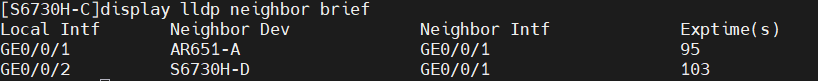
\includegraphics[scale= 0.9]{Pictures/LLD2.png}
    \caption{Confirmación de vecinos de LLDP en el switch C}
    
\end{figure}

\begin{figure}[H]
    \centering
    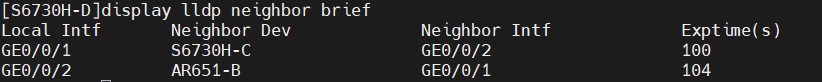
\includegraphics[scale= 0.9]{Pictures/LLD3.png}
    \caption{Confirmación de vecinos de LLDP en el switch D}
    
\end{figure}



\item Paso 3: configurar snmp\_topology

Netdata tiene un colector independiente llamado snmp\_topology. Este toma automáticamente los dispositivos definidos en:
\begin{lstlisting}[style=terminal]
/etc/netdata/go.d/snmp.conf
\end{lstlisting}

Abrir:
\begin{lstlisting}[style=terminal]
sudo nano /etc/netdata/go.d/snmp_topology.conf
\end{lstlisting}



Contenido del archivo:

\begin{lstlisting}[style=terminal]
jobs:
  - name: snmp_topology
    update_every: 10
    refresh_every: 1m


\end{lstlisting}


Los parámetros significan:

\begin{itemize}
     

\item update\_every: 10: revisa cada 10 segundos si hay dispositivos nuevos o eliminados.
\item refresh\_every: 1m: vuelve a consultar la topología cada minuto.


\end{itemize}


El valor predeterminado de refresh\_every es 30 minutos, por lo que para el laboratorio conviene reducirlo temporalmente a un minuto. El mínimo permitido para update\_every es 10 segundos. \cite{netdata-documentacion}


\item Luego de esto, se debe reiniciar el servicio de Netdata para que los cambios surtan efecto:
\begin{lstlisting}[style=terminal]
sudo systemctl restart netdata
\end{lstlisting}


\begin{lstlisting}[style=terminal]
sudo journalctl \
  _SYSTEMD_INVOCATION_ID="$(systemctl show --value --property=InvocationID netdata)" \
  --namespace=netdata \
  --no-pager |
grep -iE 'snmp_topology|topology|lldp|collector=snmp|error'

\end{lstlisting}



\end{itemize}